We compute the upper limits using the shape of the LR to maximize the analysis sensitivity as described in 
Section~\ref{sec:results}. The expected upper limit at 95\%C.L correspoinding to 1~$\ifb$ 
as a function of $m_H$ using the LR are shown in Figure~\ref{fig:me_expected_1fb} 
comparing the corresponding results using the BDT output. 
In the calculation, we apply overal data-to-simualtion scale factors to the yields predictd by simulation.  
%The scale factor for the SM Higgs is 1.13, 1.9 for the $\ttbar+tW$ and $\Wjets$, and 2.6 $\dyll+WZ+ZZ$. 
The sensitivity performance of the matrix element method is consistent with the BDT based approach.
% with a slightly larger exclusion region. 
The results for each mass points are tabulated in Table~\ref{tab:me_expected_1fb}. 

%%%%%%%%%%%%%%%%%%%%%%%%%%%%%%
\begin{figure}[!hbtp]
\centering
\subfigure[]{
\centering
\label{subfig:me_exp_1fb}
%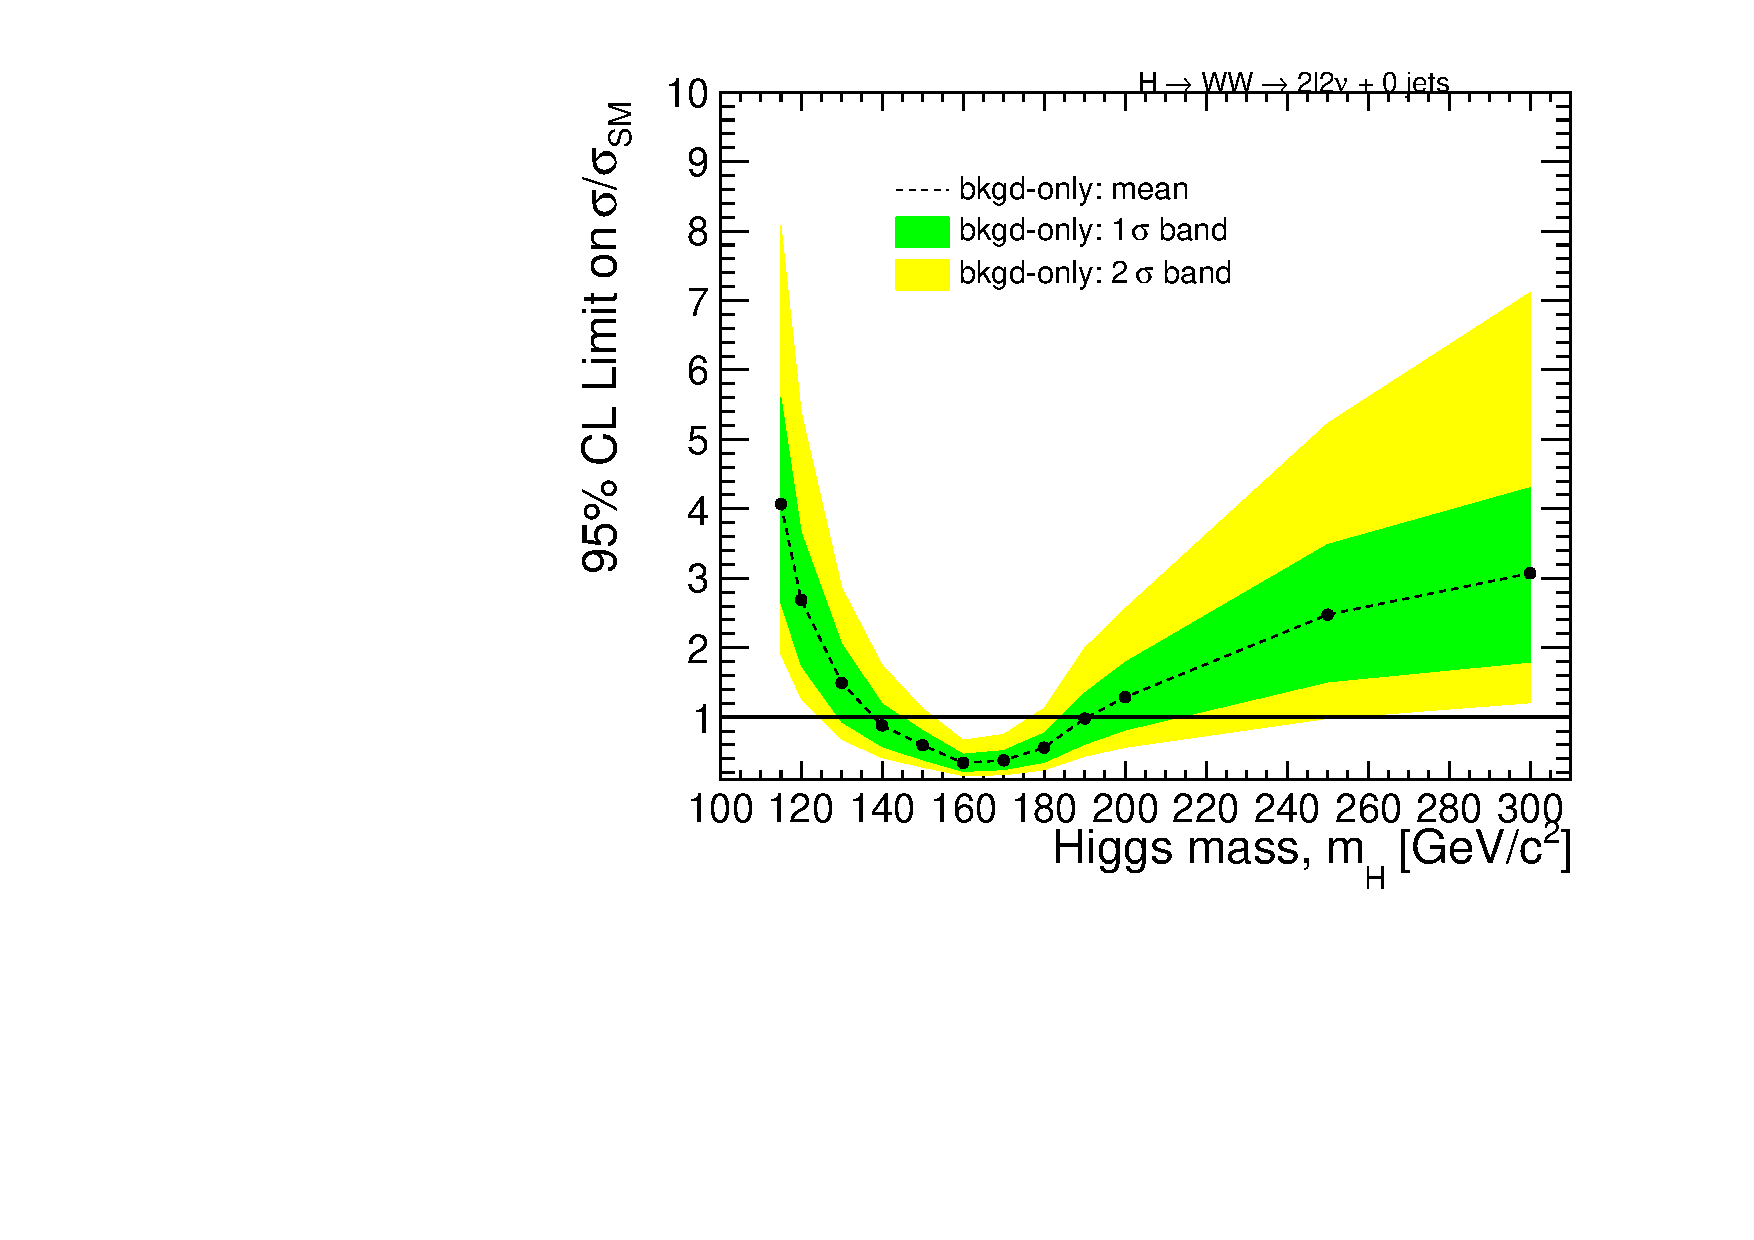
\includegraphics[width=.45\textwidth]{figures/limits_0j_1000pb_ME_shape.pdf}
}
\subfigure[]{
\centering
\label{subfig:bdt_exp_1fb}
%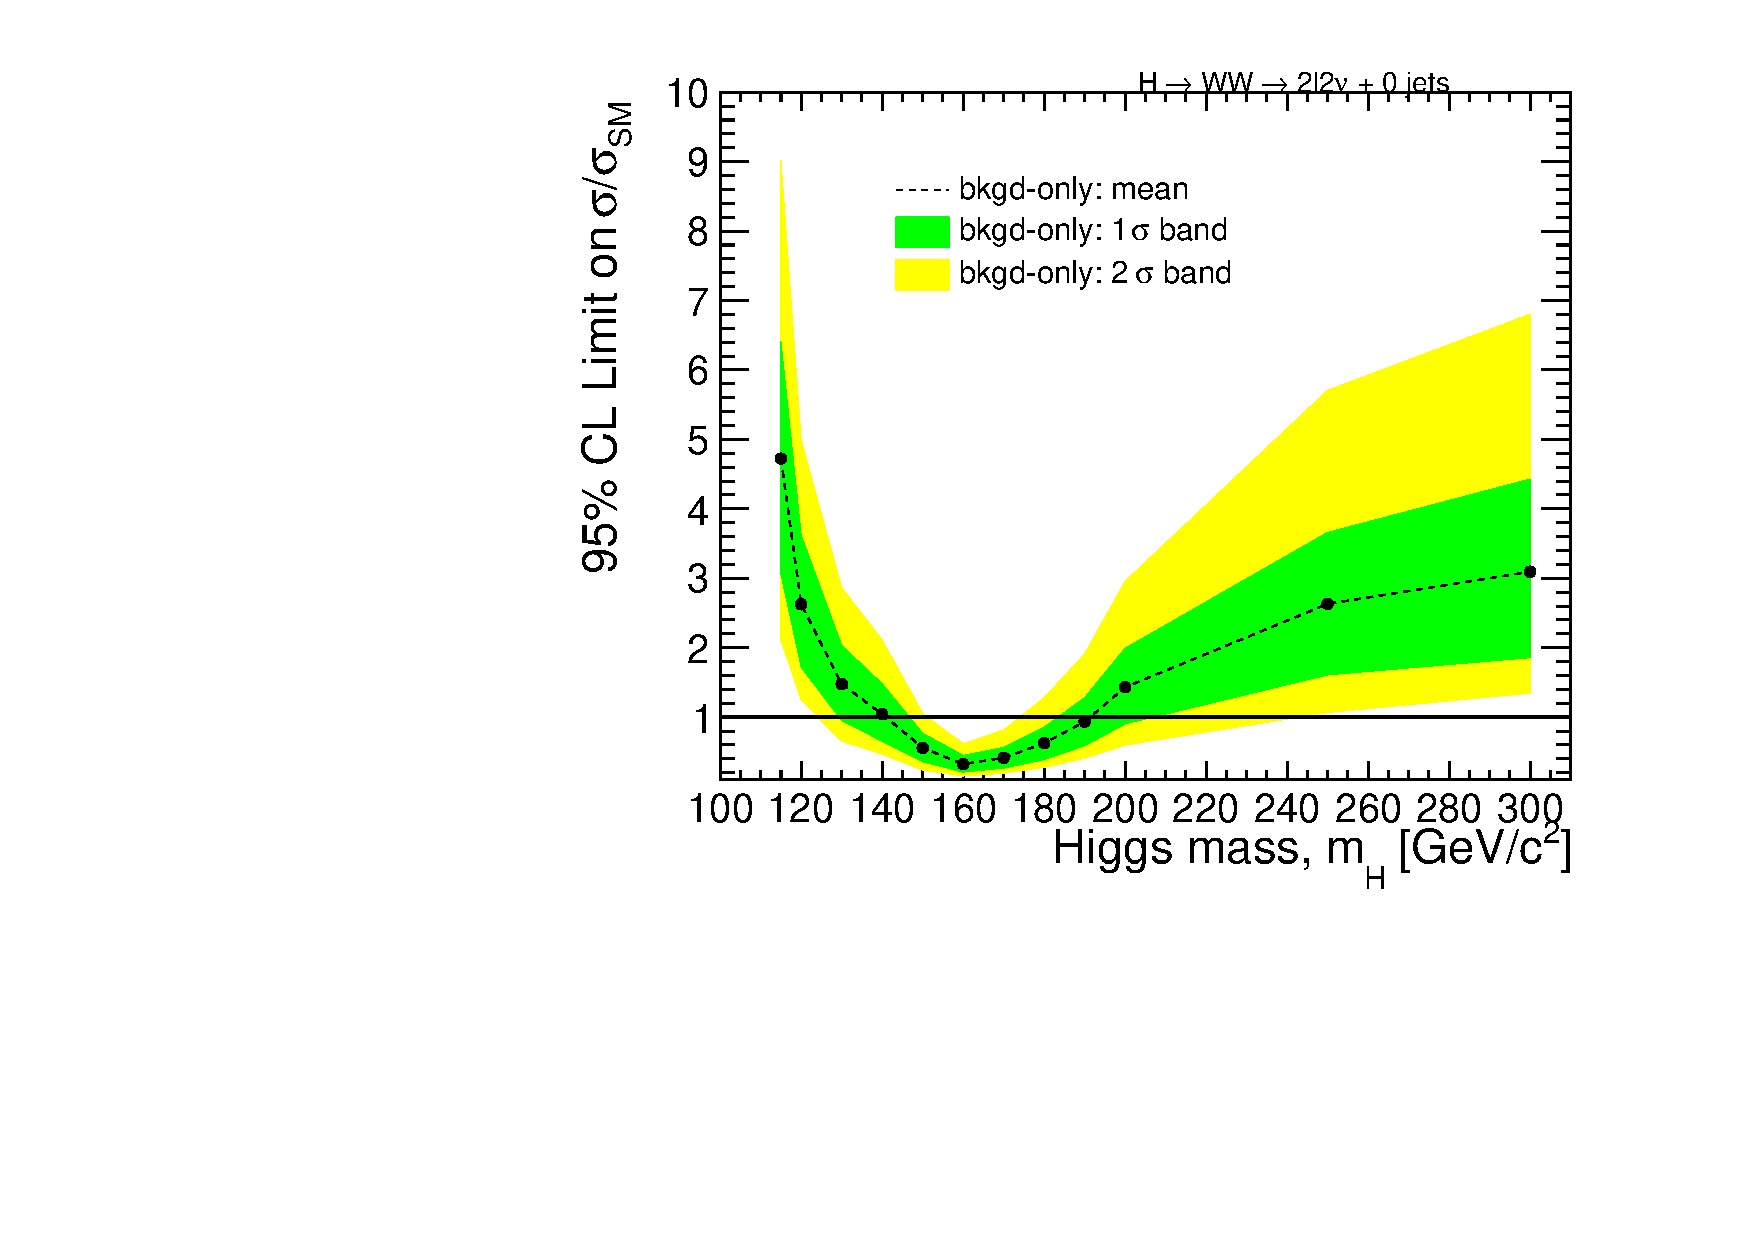
\includegraphics[width=.45\textwidth]{figures/limits_0j_1000pb_BDT_shape.pdf}} \\
}
\caption{ 
Multivariate shape analysis expected upper limits at 95\% C.L. for 1~$\ifb$ data using the 
matrix elemement output \subref{subfig:me_exp_1fb} and BDT output \subref{subfig:bdt_exp_1fb}. } 
\label{fig:me_expected_1fb}
\end{figure}
%%%%%%%%%%%%%%%%%%%%%%%%%%%%%%

%%%%%%%%%%%%%%%%%%%%%%%%%%%%%%
\begin{table}
\begin{center}
\begin{tabular}{c c c c c c c}
\hline\hline
 $m_H$ (GeV) & $-2\sigma$ & $-\sigma$ & median & $+1\sigma$ & $+2\sigma$ \\
\hline
\multicolumn{6}{c} {Cut-Based Method} \\
\hline
 200 & - & - &  - &  - &  - \\
 250 & - & - &  - &  - &  - \\
 300 & - & - &  - &  - &  - \\
 400 & - & - &  - &  - &  - \\
\hline
\multicolumn{6}{c} {Matrix Element Method} \\
\hline
 200 & - & - &  - &  - &  - \\
 250 & - & - &  - &  - &  - \\
 300 & - & - &  - &  - &  - \\
 400 & - & - &  - &  - &  - \\
\hline
\multicolumn{6}{c} {BDT Based} \\
\hline
 200 & - & - &  - &  - &  - \\
 250 & - & - &  - &  - &  - \\
 300 & - & - &  - &  - &  - \\
 400 & - & - &  - &  - &  - \\
\hline\hline
\end{tabular}
\end{center}
\caption{ {\bf Placeholder for results}. Multivariate shape analysis expected upper limits at 95\% C.L. for 1~$\ifb$ data using the 
matrix elemement and BDT output corresponding to Figure~\ref{fig:me_expected_1fb}.}
\label{tab:me_expected_1fb}
\end{table}
%%%%%%%%%%%%%%%%%%%%%%%%%%%%%%